\chapter{Arhitektura i dizajn sustava}

\begin{figure}[H]
	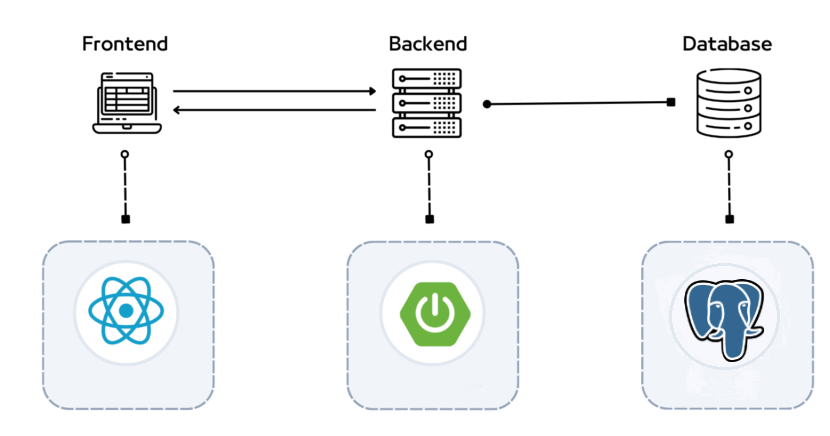
\includegraphics[scale=1]{slike/prikaz_arhitekture.png}
	\centering
	\caption{Prikaz arhitekture sustava}
\end{figure}

Arhitektura sustava može se podijeliti na tri glavna podsustava, a to su \textbf{Web poslužitelj, Web aplikacija i baza podataka}.
\begin{itemize}
	\item 	\textit{\textbf{Web poslužitelj}} prima zahtjeve od klijenata putem interneta, obrađuje ih i pruža resurse poput web stranice, slike, videa i datoteke kao odgovor. Za distribuciju resursa najčešče se koriste protokoli kao što su HTTP (Hypertext Transfer Protocol) ili HTTPS (HTTP Secure).
	\item 	\textit{\textbf{Web aplikacija}} je program koji se izvršava na web pregledniku (Google Chrome, Mozilla Firefox, Safari itd.) i pruža korisnicima mogućnost izvršavanja željenih zahtjeva, odnosno interakciju s određenim uslugama i funkcionalnostima web aplikacije. Prilikom obrade zahtjeva pristupa se bazi podataka i korisniku se odgovor vraća kao HTML dokument.
	\item 	\textit{\textbf{Baza podataka}} je organizirani skup podataka namijenjen za efikasno upravljanje, ažuriranje, pretraživanje i dohvat podataka. Uloge baze podataka u web aplikaciji su pohrana podataka, očuvanje integriteta podataka i osiguravanje dosljednosti, upravljanje transakcijama itd.
\end{itemize}

Za izradu naše web aplikacije odabrali smo \textit{\textbf{Spring Boot}} (open-source Java framework) i \textit{\textbf{React}} (open-source JavaScript library). Odabrana razvojna okruženja su InteliJ IDEA i Eclipse IDE za Spring Boot, odnosno Visual Studio Code i WebStorm za React. Za izradu baze podatka koristimo PostgreSQL.
Arhitektura, koja je podržana Spring Boot-om, temelji se na \textit{\textbf{MVC (Model-View-Controller)}} konceptu koji strogo odvaja model, akcije i prezentaciju, olakšava razvoj i održavanje aplikacije te čini aplikaciju prilagodljivom i jednostavnom za proširenje.
\begin{itemize}
	\item \textit{\textbf{Model}} - predstavlja poslovnu logiku, odnosno dinamičke strukture podataka, mijenja pogled na zahtjev kontrolera. Modeli u pravilu predstavljaju podatke(objekte) koje aplikacija obrađuje.
	\item \textit{\textbf{View}} - ono što klijent vidi, odnosno korisničko sučelje potrebno za interakciju s aplikacijom kao što su dijagrami, linkovi, slike, tablice itd.
	\item \textit{\textbf{Controller}} - presreće zahtjeve klijenata i prilagođava model, odnosno obavještava model o promjeni zahtjeva korisnika i u skladu sa zahtjevima daje prikladan View.
\end{itemize}

\section{Baza podataka}
			
Za potrebe našeg sustava koristit ćemo relacijsku bazu podataka koja svojom strukturom olakšava modeliranje stvarnog svijeta. Gradivna jedinka baze je relacija, od- nosno tablica koja je definirana svojim imenom i skupom atributa. Zadaća baze podataka je brza i jednostavna pohrana, izmjena i dohvat podataka za daljnju obradu. Baza podataka ove aplikacije sastoji se od sljedećih entiteta:
\begin{itemize}
	\item Natjecanje
	\item VirtualnoNatjecanje
	\item Korisnik
	\item Uloga
	\item Pehar
	\item Zadatak
	\item Rješenje
	\item TestniPrimjer		
\end{itemize}
				
\subsection{Opis tablica}
			

\textbf{Natjecanje} \quad Ovaj entiet sadržava informacije o natjecanju koje trenutno rješava korisnik. Atributi koje sadržava su: NatjecanjeID, VoditeljID, NazivNatjecanja, PocetakNatjecanja, ZavršetakNatjecanja. Ovaj entitet ima  \textit{One-to-Many} vazu s entitetom Pehar preko atributa NatjecanjeID, te  \textit{One-to-Many} vezu sa slabim entitetom VirtualnoNatjecanje preko atributa OriginalnoNajtecanjeID. Ima  \textit{One-to-Many} vezu s entitetom Korisnik preko atributa VoditeljID.
				
				
				\begin{longtblr}[
					label=none,
					entry=none
					]{
						width = \textwidth,
						colspec={|X[9,l]|X[6, l]|X[18, l]|}, 
						rowhead = 1,
					} %definicija širine tablice, širine stupaca, poravnanje i broja redaka naslova tablice
					\hline \SetCell[c=3]{c}{\textbf{Natjecanje}}	 \\ \hline[3pt]
					\SetCell{LightGreen}NatjecanjeID & INT	&  	Jedinstveni identifikator natjecanja  	\\ \hline
					\SetCell{LightBlue}VoditeljID	& INT &  Jedinstveni identifikator voditelja 	\\ \hline 
					NazivNatjecanja & VARCHAR &  Naziv natjecanja \\ \hline 
					PocetakNatjecanja & TIMESTAMP	&  	Vrijeme početka natjecanja	\\ \hline 
					ZavrsetakNatjecanja	& TIMESTAMP &   Vrijeme završetka natjecanja	\\ \hline 
				\end{longtblr}
				
\textbf{VirtualnoNatjecanje} \quad Ovaj enitet sadržava informacije o virtualnom natjecanju koje je pokrenuo korisnik na temelju nekog natjecanja. Atributi koje sadržava su: virtualnoNatjecanjeID, natjecateljID i originalnoNatjecanjeID. Ovaj entitet ima \textit{Many-To-One} vezu s entitetom korisnik preko atributa i vanjskog ključa korisnikID. Atribut originalnoNatjecanjeID predstavlja vanjski ključ koji se referencira na natjecanjeID u relaciji natjecanje pa se time tvori \textit{Many-To-One} veza.
		
				\begin{longtblr}[
					label=none,
					entry=none
					]{
						width = \textwidth,
						colspec={|X[11,l]|X[3, l]|X[20, l]|}, 
						rowhead = 1,
					} %definicija širine tablice, širine stupaca, poravnanje i broja redaka naslova tablice
					\hline \SetCell[c=3]{c}{\textbf{VirtualnoNatjecanje}}	 \\ \hline[3pt]
					\SetCell{LightGreen}VirtualnoNatjecanjeID & INT & Jedinstveni identifikator virtualnog natjecanja  	\\ \hline
					\SetCell{LightBlue}natjecateljID & INT &  ID korisnika koji je stvorio virtualno natjecanje \\ \hline
					\SetCell{LightBlue}originalnoNatjecanjeID & INT &  ID natjecanja na kojem se temelji virtualno natjecanje 	\\ \hline  
				\end{longtblr}

\textbf{Korisnik} \quad Ovaj entitet sadržava sve bitne informacije o korisniku aplikacije. Sadrži atribute: KorisnickoIme, lozinka, ime, prezime, email, fotografija, vrijemeRegistracije te ulogaID. Ovaj entitet je u vezi \textit{One-to-Many} s entitetom Natjecanje preko atributa VoditeljID, u vezi  \textit{One-to-Many} s entitetom Zadatak preko atributa VoditeljID, u vezi  \textit{One-to-Many} s entitetom Rjesenje preko atributa NatjecateljID, te je u  \textit{One-to-Many} s entitetom Pehar preko atributa NatjecateljID. Entitet ima  \textit{Many-to-One} vezu s entitetom Uloga preko atribura UlogaID.
				
				\begin{longtblr}[
					label=none,
					entry=none
					]{
						width = \textwidth,
						colspec={|X[9,l]|X[6, l]|X[18, l]|}, 
						rowhead = 1,
					} %definicija širine tablice, širine stupaca, poravnanje i broja redaka naslova tablice
					\hline \SetCell[c=3]{c}{\textbf{Korisnik}}	 \\ \hline[3pt]
					\SetCell{LightGreen}KorisnikID & INT	&  	Jedinstveni identifikator korisnika  	\\ \hline
					KorisničkoIme	& VARCHAR &  Jedinstveno ime korisnika 	\\ \hline 
					Lozinka & VARCHAR &  Korisnikova lozinka \\ \hline 
					Ime & VARCHAR	&  	Ime korisnika	\\ \hline 
					Prezime	& VARCHAR &   Prezime korisnika	\\ \hline 
					Email & VARCHAR & elektronička pošta korisnika \\ \hline 
					Fotografija & PATH & fotografija korisnika \\ \hline 
					VrijemeRegistracije & TIMESTAMP & Vrijeme kada se korisnik registrirao u sustav \\ \hline 
					\SetCell{LightBlue}UlogaID & INT & Jedinstveni identifikator uloge	\\ \hline
				\end{longtblr}
				
\textbf{Uloga} \quad Ovaj entitet predstavlja ulogu koju korisnik može poprimiti. Sadrži atribute UlogaID te UlogaNaziv. Ima  \textit{One-to-Many} vezu s entitetom Korisnik preko atributa UlogaID.
				
				\begin{longtblr}[
					label=none,
					entry=none
					]{
						width = \textwidth,
						colspec={|X[9,l]|X[6, l]|X[18, l]|}, 
						rowhead = 1,
					} %definicija širine tablice, širine stupaca, poravnanje i broja redaka naslova tablice
					\hline \SetCell[c=3]{c}{\textbf{Uloga}}	 \\ \hline[3pt]
					\SetCell{LightGreen}UlogaID & INT	&  	Jedinstveni identifikator uloge  	\\ \hline
					UlogaNaziv	& VARCHAR &  Naziv uloge 	\\ \hline 
				\end{longtblr}
				
\textbf{Pehar} \quad Ovaj entitet predstavlja pehar kojeg natjecatelji (korisnici) mogu osvojiti u natjecanju. Sadrži atribute: PeharID, NatjecateljID, NatjecanjeID, Mjesto te SlikaPehara. Ovaj entitet ima  \textit{Many-to-One} vezu s entitetom Natjecanje preko atributa NatjecanjeID, te ima vezu  \textit{Many-to-One} s entitetom Korisnik preko atributa NatjecateljID.
				
				\begin{longtblr}[
					label=none,
					entry=none
					]{
						width = \textwidth,
						colspec={|X[9,l]|X[4, l]|X[20, l]|}, 
						rowhead = 1,
					} %definicija širine tablice, širine stupaca, poravnanje i broja redaka naslova tablice
					\hline \SetCell[c=3]{c}{\textbf{Pehar}}	 \\ \hline[3pt]
					\SetCell{LightGreen}PeharID & INT	&  	Jedinstveni identifikator pehara  	\\ \hline
					\SetCell{LightBlue}NatjecateljID	 & INT &  Jedinstveni identifikator natjecatelja 	\\ \hline 
					\SetCell{LightBlue}NatjecanjeID & INT &  Jedinstveni identifikator natjecanja	\\ \hline 
					Mjesto & INT & Mjesto koje je dobiveno peharom (1, 2 ili 3) \\ \hline
					SlikaPehara & PATH & Slika dobivenog pehara \\ \hline
				\end{longtblr}

\textbf{Zadatak} \quad Ovaj enitet sadržava sve bitne značajke za definiciju jednog zadataka u aplikaciji. Atributi koje sadržava su: zadatakID, natjecanjeID, voditeljID, nazivZadatka, brojBodova, vremenskoOgranicenje, tekstZadatka te privatniZadatak. Ovaj entitet ima \textit{One-To-Many} vezu sa slabim entitetom testniPrimjer preko atributa zadatakID. Vanjskim ključem natjecanjeID stvorena je opcionalna \textit{Many-To-One} veza sa entitetom natjecanje. Postoji i \textit{One-To-Many} veza s entitetom rješenje preko atributa zadatakID. \textit{Many-To-One} veza postoji i sa entitetom korisnik preko vanjskog ključa voditeljID (označava identifikator korisnika s ulogom voditelja).
				
				\begin{longtblr}[
					label=none,
					entry=none
					]{
						width = \textwidth,
						colspec={|X[10,l]|X[6, l]|X[18, l]|}, 
						rowhead = 1,
					} %definicija širine tablice, širine stupaca, poravnanje i broja redaka naslova tablice
					\hline \SetCell[c=3]{c}{\textbf{Zadatak}}	 \\ \hline[3pt]
					\SetCell{LightGreen}ZadatakID & INT	&  	Jedinstveni  privatni identifikator zadatka  	\\ \hline
					\SetCell{LightBlue}NatjecanjeID	 & INT &  Jedinstveni identifikator natjecanja kojem pripada zadatak	\\ \hline 
					nazivZadatka & VARCHAR & Naziv zadatka \\ \hline
					tekstZadatka & TEXT & tekst kojim je zadan zadatak \\ \hline
					brojBodova & INT & broj bodova koliko nosi zadatak \\ \hline
					vremenskoOgranicenje & INT & vremensko ograničenje za izvođenje predanog rješenja \\ \hline
					privatniZadatak & BOOLEAN & zastavica koja određuje ako je zadatak privatan \\ \hline
					\SetCell{LightBlue}VoditeljD & INT &  Jedinstveni identifikator voditelja koji je stvorio zadatak	\\ \hline 
				\end{longtblr}
				
				
\textbf{Rješenje} \quad Ovaj slabi enitet sadržava informacije o predenim rješenjima pojedinog korisnika za određeni zadatak. Atributi koje sadržava su: rješenjeRb, natjecateljID, zadatakID, vrijemeOdgovora, brojTočnihPrimjera, brojBodova i programskiKod. Ovaj entitet ima \textit{Many-To-One} vezu s  entitetom zadatak preko atributa i vanjskog ključa zadatakID. \textit{Many-To-One} veza postoji i sa entitetom korisnik preko vanjskog ključa korisnikID.
				
				\begin{longtblr}[
					label=none,
					entry=none
					]{
						width = \textwidth,
						colspec={|X[10,l]|X[6, l]|X[18, l]|}, 
						rowhead = 1,
					} %definicija širine tablice, širine stupaca, poravnanje i broja redaka naslova tablice
					\hline \SetCell[c=3]{c}{\textbf{Rješenje}}	 \\ \hline[3pt]
					\SetCell{LightGreen}rjesenjeRb & INT & Redni broj predanog rješenja određenog korisnika za predani zadatak \\ \hline
					\SetCell{LightBlue}ZadatakID & INT	&  	Jedinstveni  privatni identifikator zadatka  	\\ \hline
					\SetCell{LightBlue}NatjecateljD & INT &  Jedinstveni identifikator natjecatelja koji je predao rješenje	\\ \hline 
					vrijemeOdgovora & TIMESTAMP & Vrijeme predaje rješenja \\ \hline
					brojTočnihOdgovora & INT & Broj primjera koji prolaze evaluaciju \\ \hline
					brojBodova & INT & Ostvareni broj bodova na zadatku \\ \hline
					programskiKod & TEXT & Programski kod predanog rješenja \\ \hline
				\end{longtblr}
				
\textbf{TesniPrimjer} \quad Ovaj slabi enitet sadržava informacije o testnim primjerima za određeni zadatak. Atributi koje sadržava su: testniPrimjerRb, zadatakID, ulazniPodaci i izlazniPodaci. Ovaj entitet ima \textit{Many-To-One} vezu s entitetom zadatak preko atributa i vanjskog ključa zadatakID.
	
				\begin{longtblr}[
					label=none,
					entry=none
					]{
						width = \textwidth,
						colspec={|X[11,l]|X[3, l]|X[20, l]|}, 
						rowhead = 1,
					} %definicija širine tablice, širine stupaca, poravnanje i broja redaka naslova tablice
					\hline \SetCell[c=3]{c}{\textbf{TestniPrimjer}}	 \\ \hline[3pt]
					\SetCell{LightGreen}TestniPrimjerRB & INT & Redni broj testnog primjera za pojedini zadatak  	\\ \hline
					\SetCell{LightBlue}zadatakID & INT &  Jedinstveni privatni identifikator zadatka \\ \hline
					ulazniPodaci & TEXT & ulazni podaci za testiranje programskog rješenja \\ \hline
					izlazniPodaci & TEXT & očekivani ispis programskog rješenja \\ \hline
				\end{longtblr}
						
		
\pagebreak
\subsection{Dijagram baze podataka}
%\textit{ U ovom potpoglavlju potrebno je umetnuti dijagram baze podataka. Primarni i strani ključevi moraju biti označeni, a tablice povezane. Bazu podataka je potrebno normalizirati. Podsjetite se kolegija "Baze podataka".}
\begin{figure}[H]
	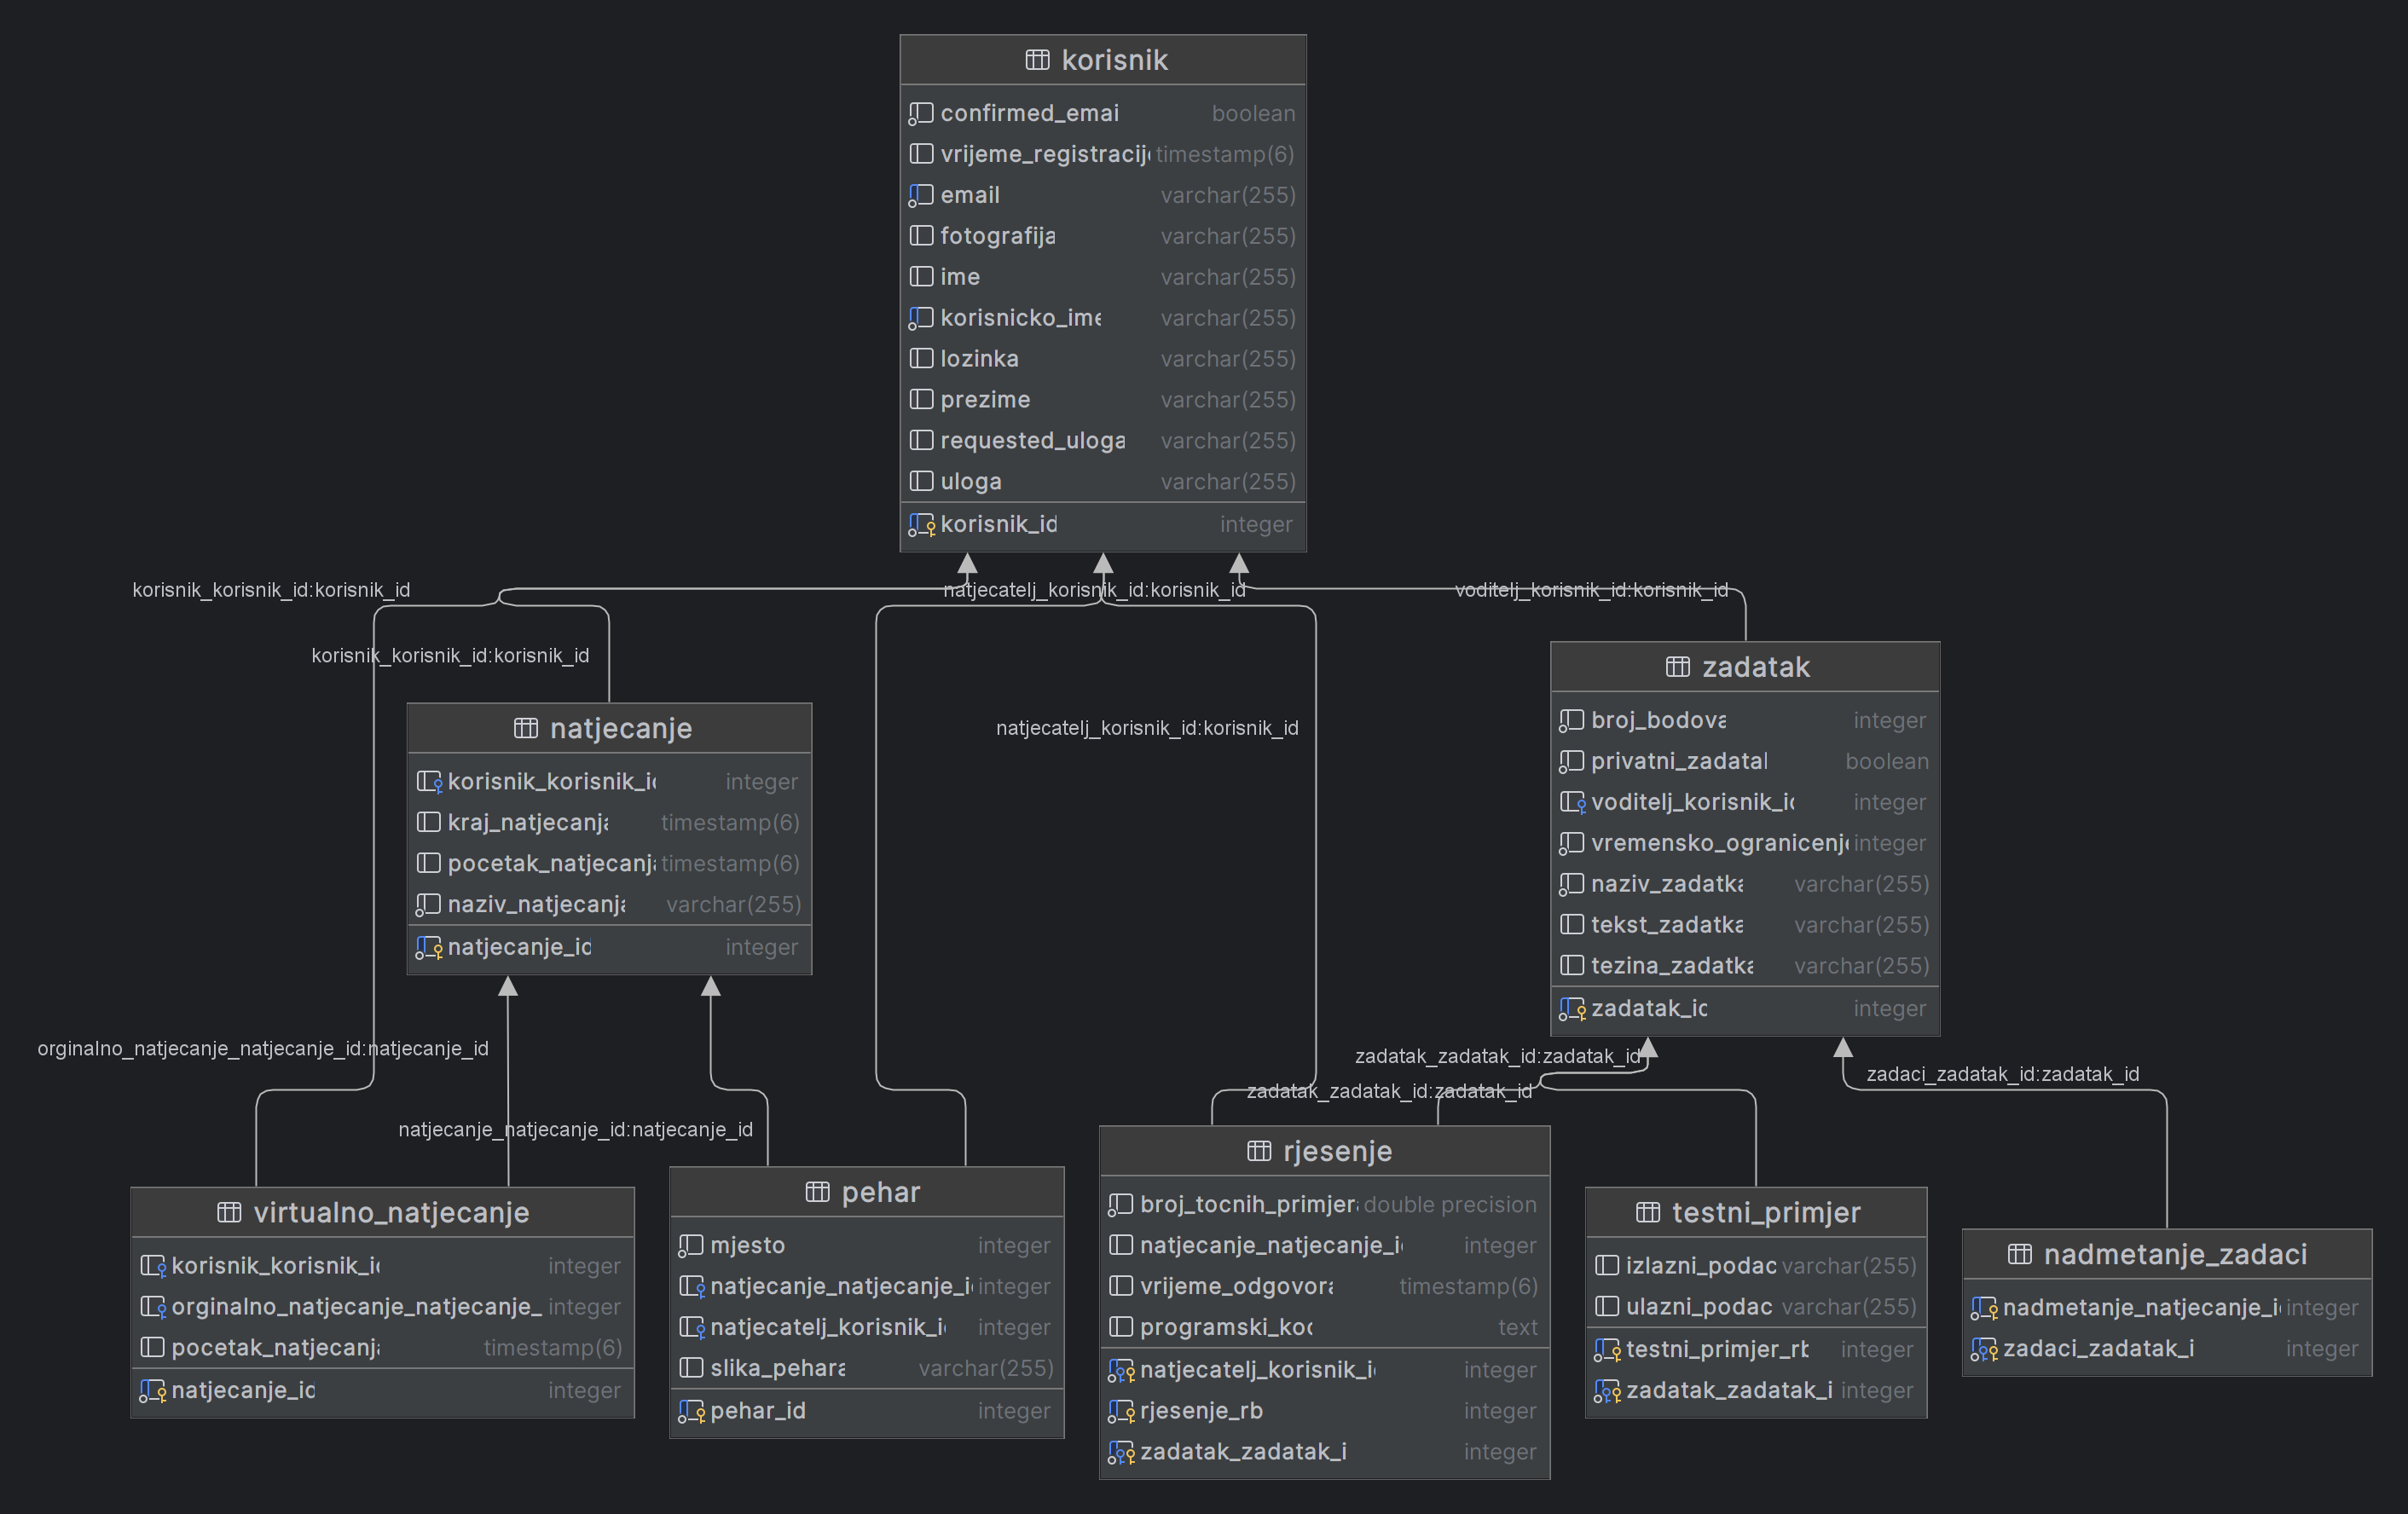
\includegraphics[scale=0.7]{dijagrami/dijagram_baze_podataka.png}
	\centering
	\caption{Dijagram baze podataka}
	\label{fig:bazaPodataka} 
\end{figure}

\eject


\section{Dijagram razreda}

Na slikama 4.3 i 4.4 prikazani su dijagrami razreda koji predstavljaju backend dio arhitekture.
Prva slika opisuje servise, odnosno njihovu implementaciju i prikazani su atributi i metode u pojedinim razredima.
Servisi predstavljaju glavnu logiku i oni su uglavnom u interakciji s repozitorijima koji su između ostalog prikazani na slici 4.4.
Osim repozitorija, na slici 4.4 prikazani su i modeli (predstavljaju strukturu baze podataka) te kontroleri. 
Kontroleri su zaduženi za upravljanje HTTP zahtjevima i pružanje prikladnog odgovora. Na drugoj slici možemo uočiti atribute i međusobne odnose prethodno navedenih razreda. \\

Razred Korisnik predstavlja registriranog korisnika koji se može registrirati kao voditelj ili natjecatelj unoseći svoje podatke u sustav.
Razred Natjecanje definira naziv, početak i kraj natjecanja te voditelja. Razred Pehar je entitet u kojeg spremamo koje mjesto je osvojio natjecatelj na nekom natjecanju i sliku pehara.
Razred uloga je enumeracija koja definira ulogu korisnika (admin, natjecatelj ili voditelj). Razred zadatak je entitet koji predstavlja određeni problem na natjecanju i sadrži referencu na testne primjere.
Testni primjer sadrži informacije o tesnim primjerima za pojedinačni zadatak. Razred Rjesenje predstavlja predano rješenje pojedinog korisnika za zadatak. 
Razred Virtualno natjecanje predstavlja natjecanje koje se može naknadno pokrenuti i rješavati. 

\begin{figure}[H]
	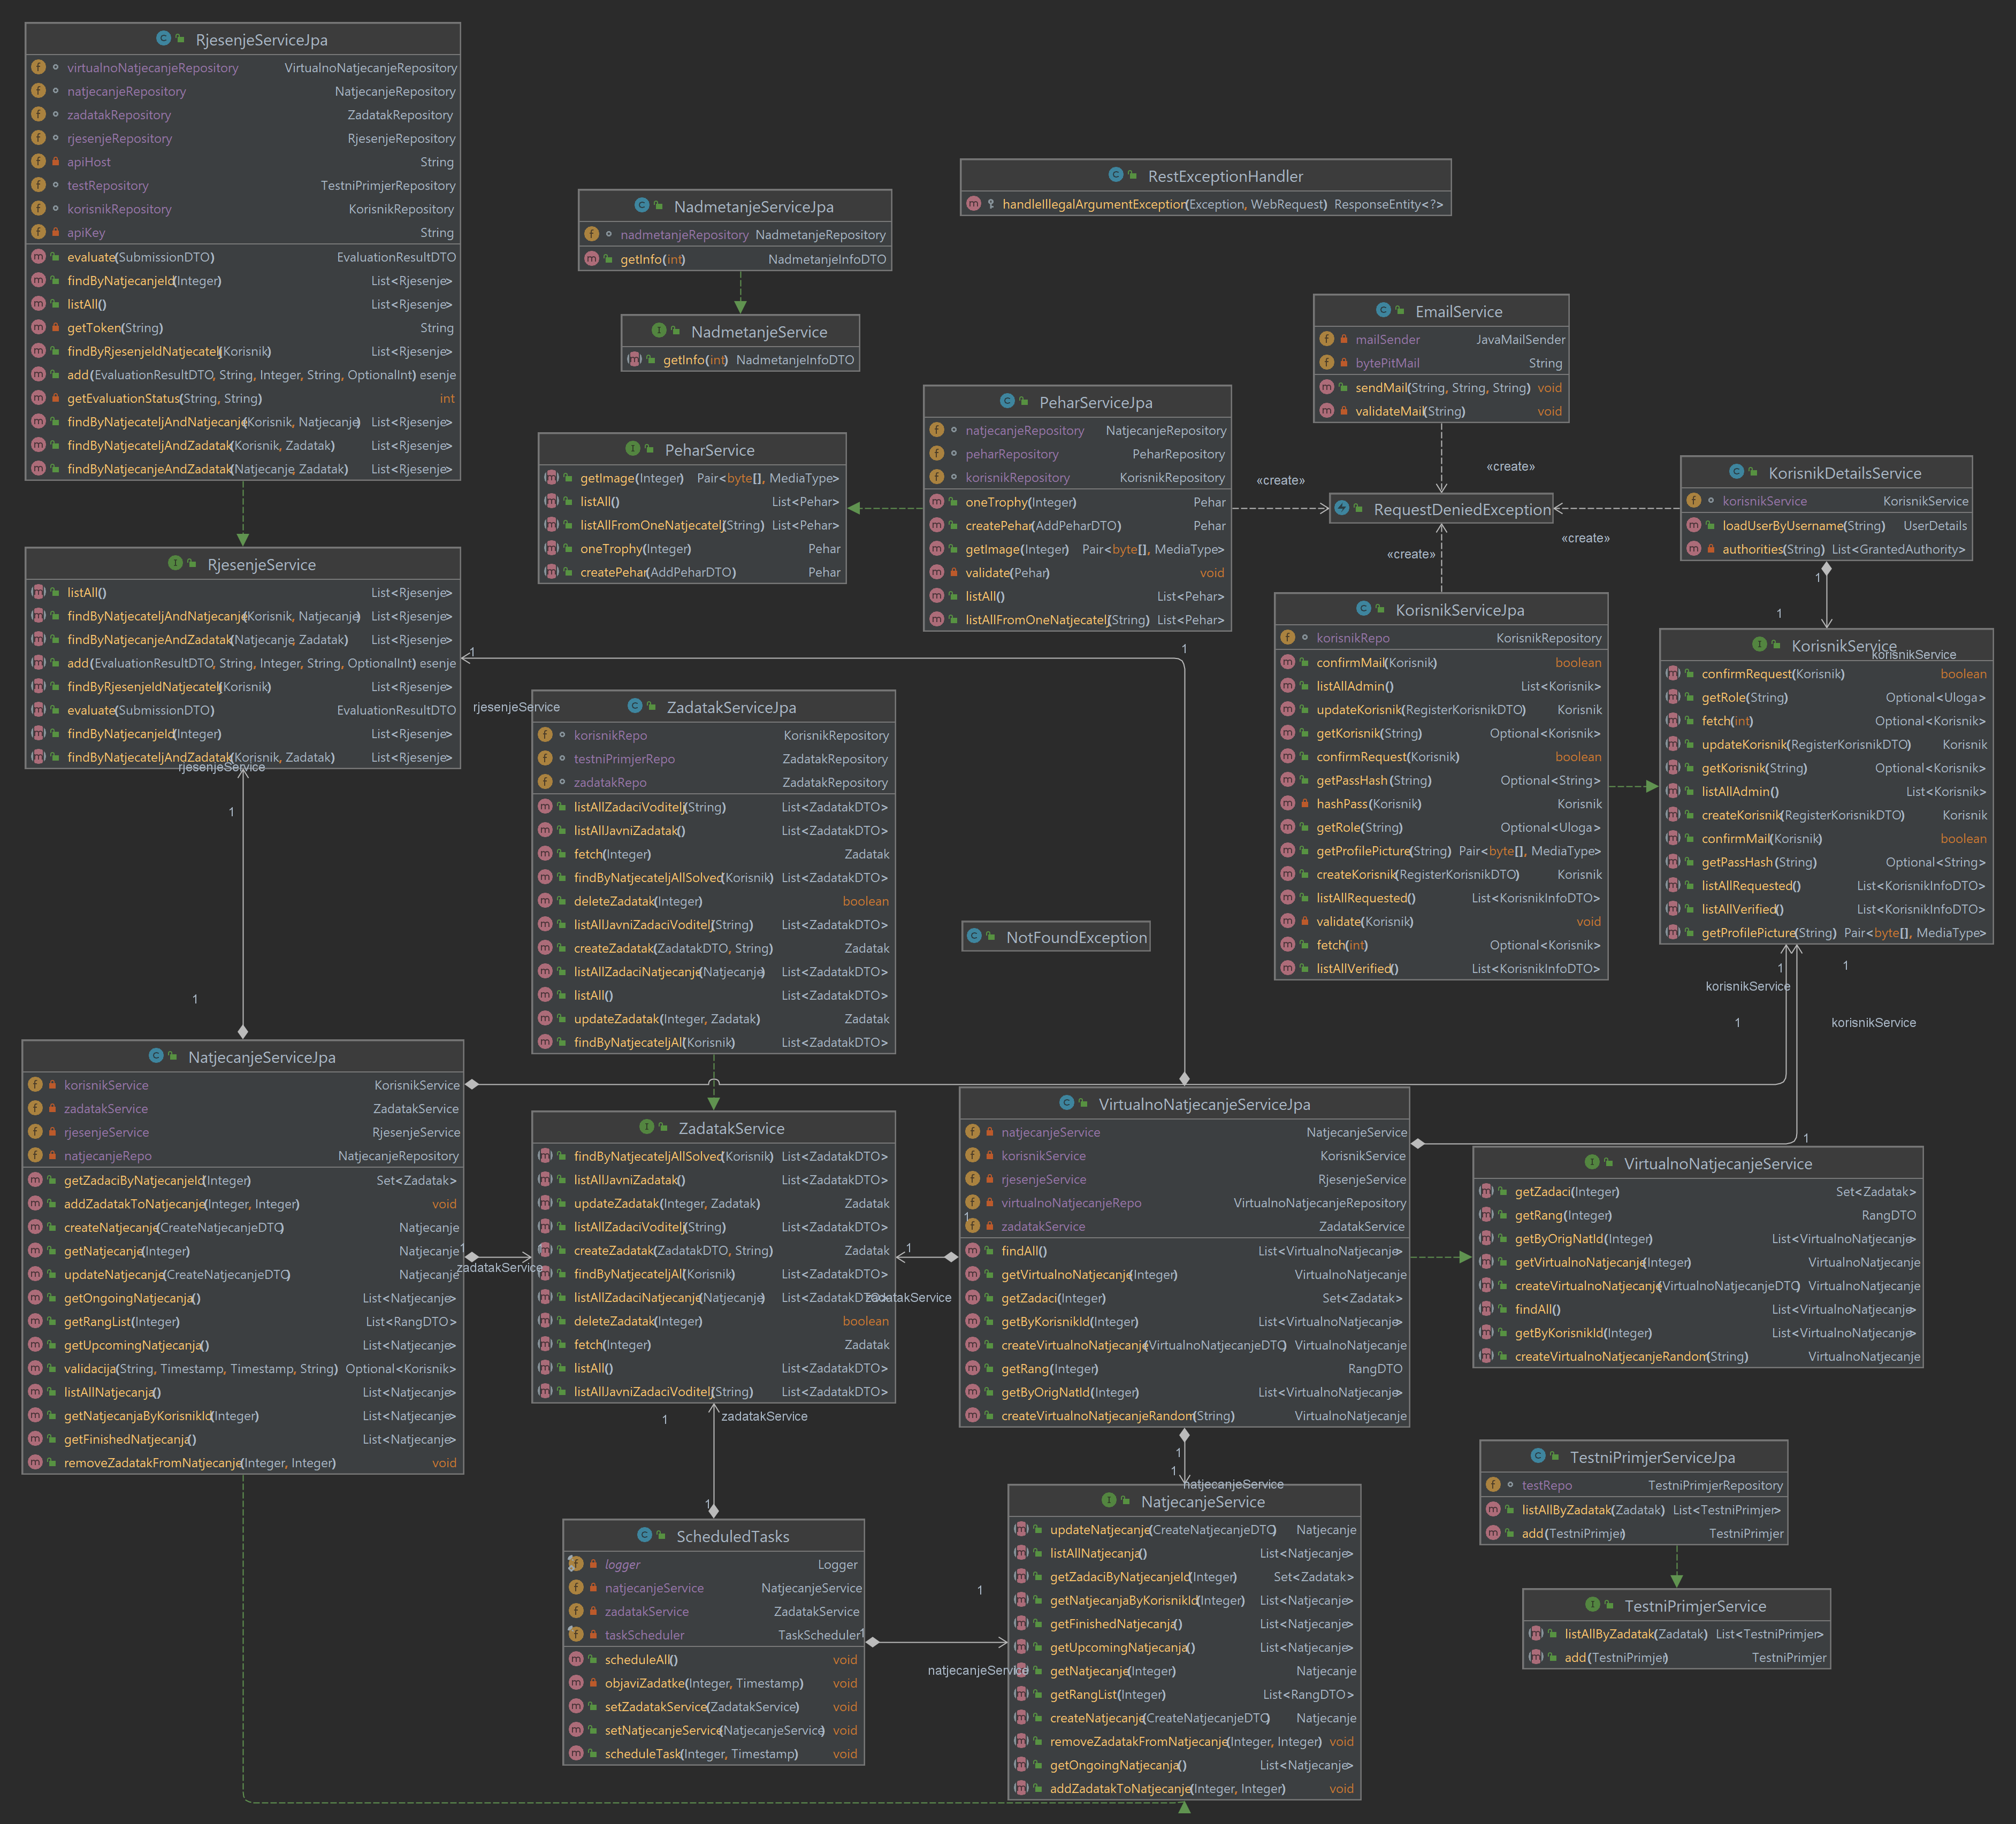
\includegraphics[scale=0.19]{dijagrami/serviceDiagram.png}
	\centering
	\caption{Dijagram razreda - Servisi}
\end{figure}

\begin{figure}[H]
	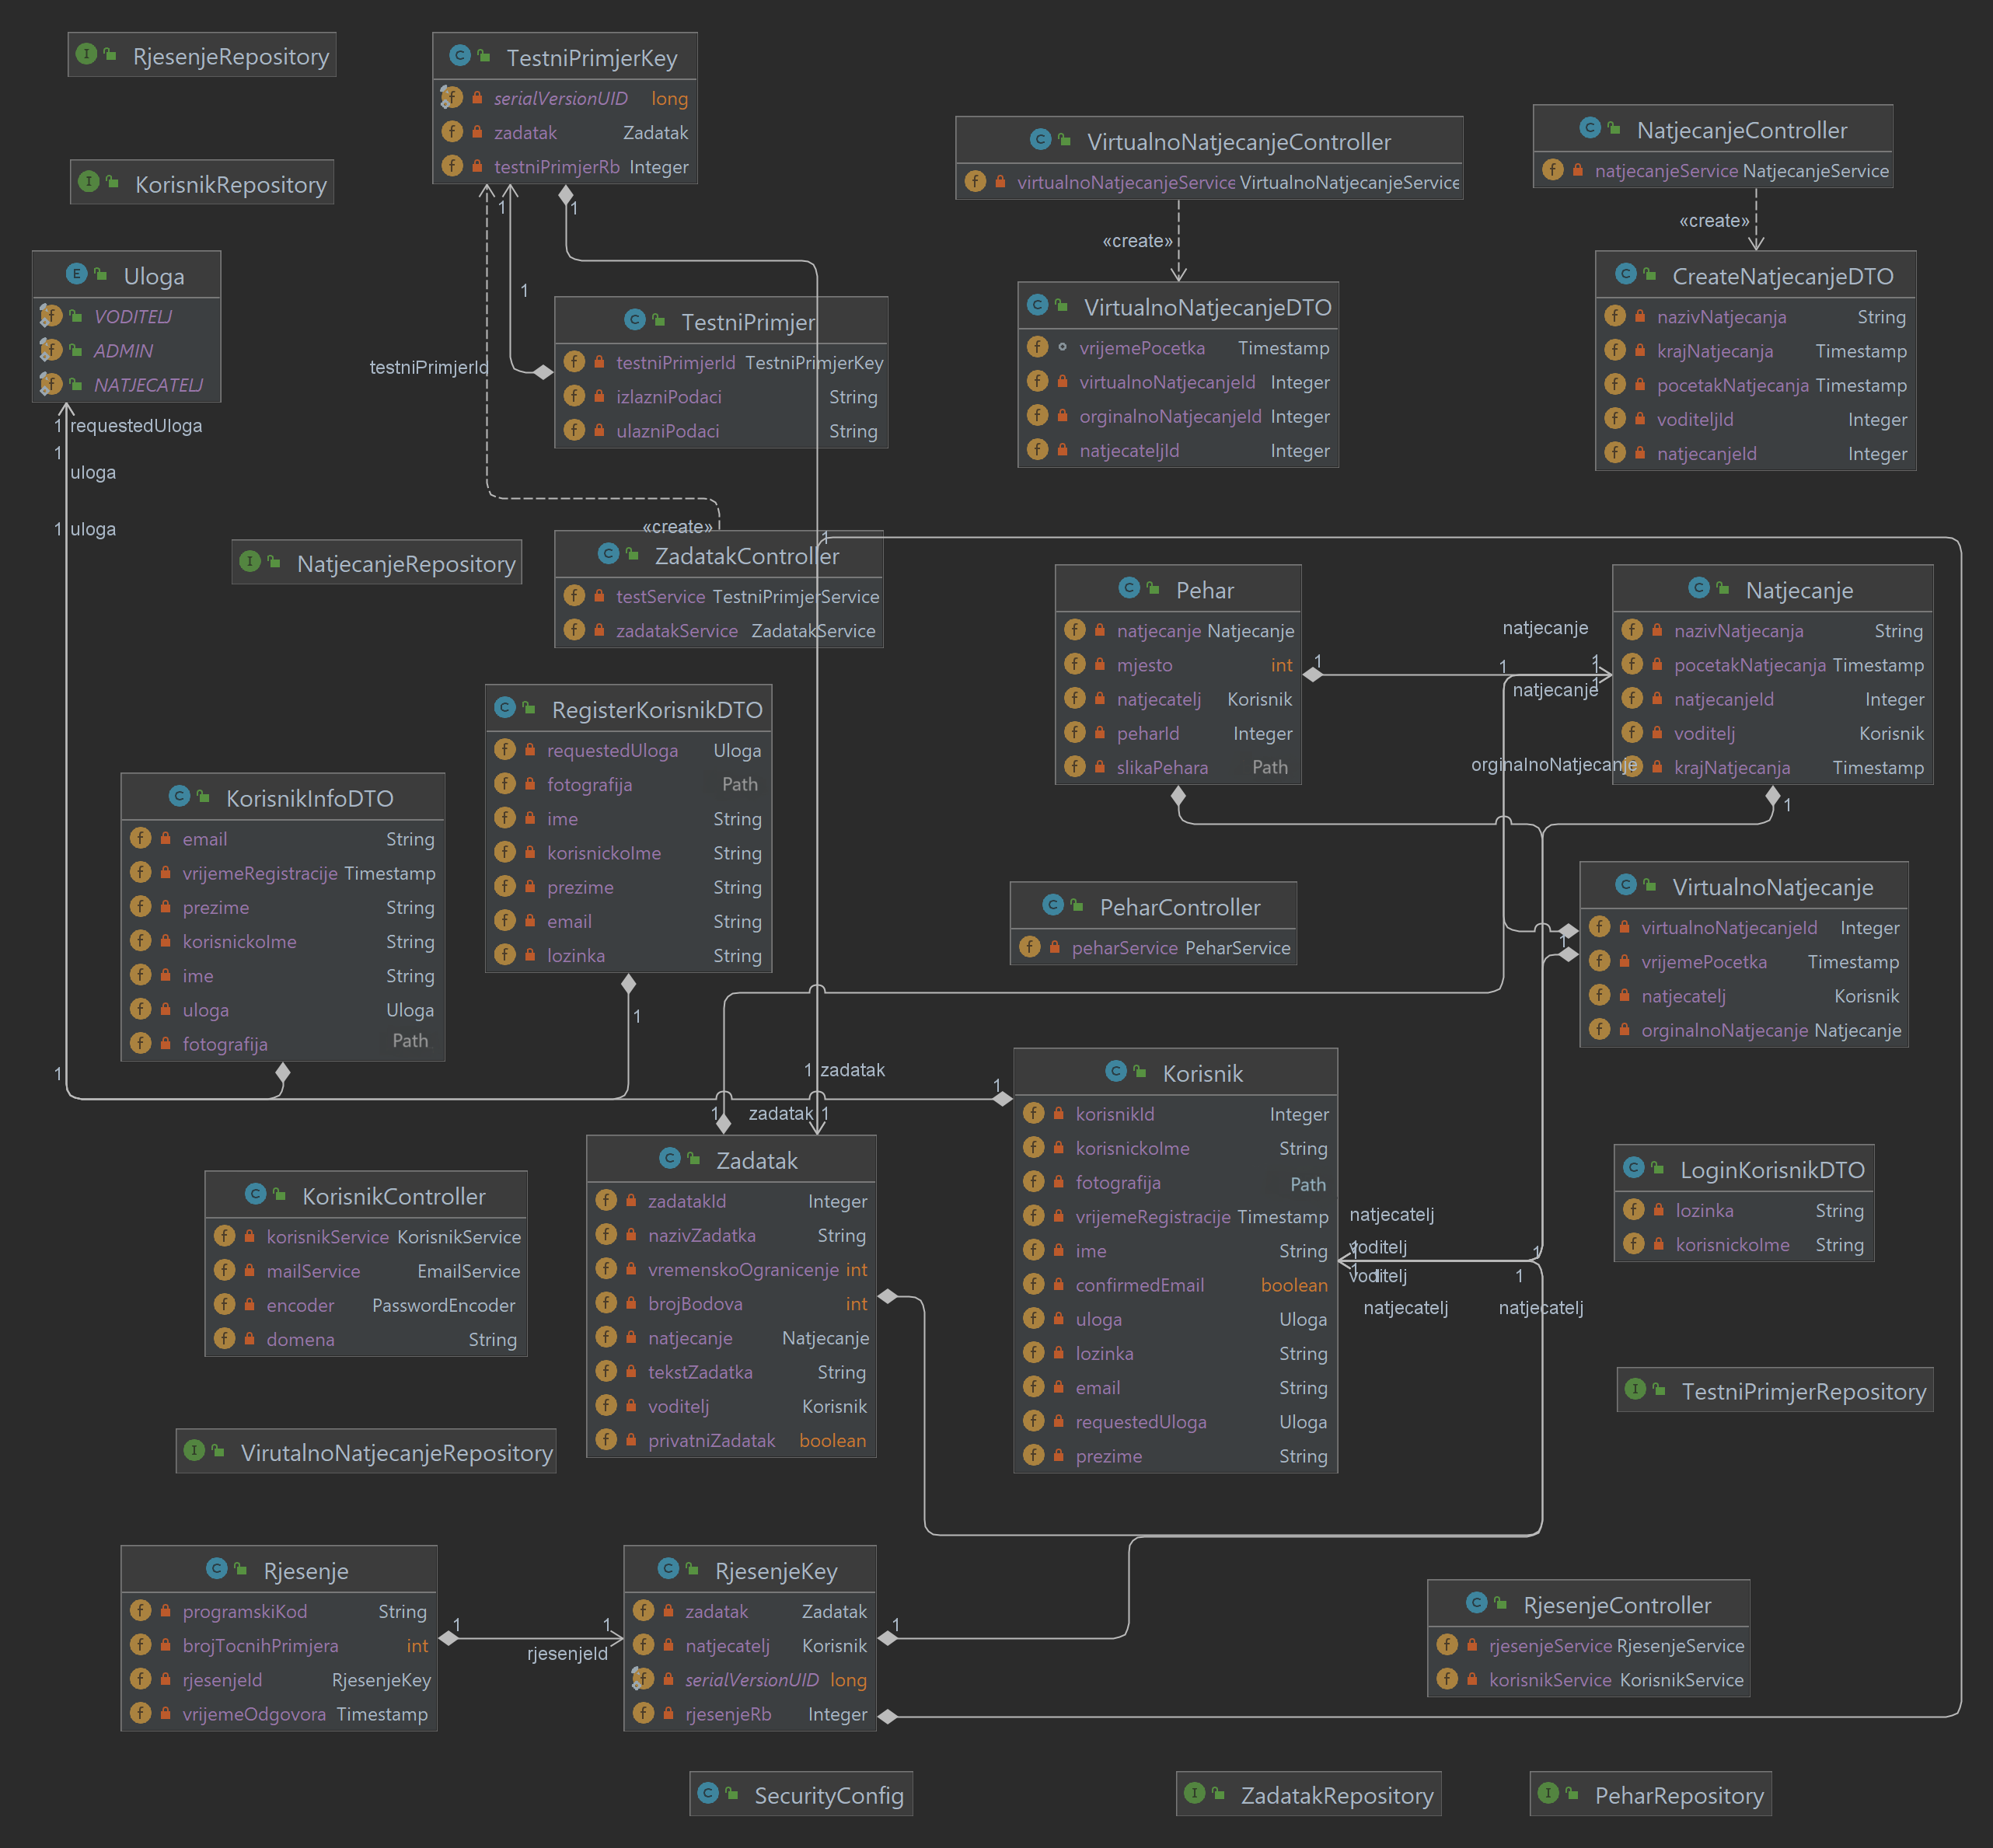
\includegraphics[scale=0.2]{dijagrami/apiDiagram.png}
	\centering
	\caption{Dijagram razreda - Kontroleri, Repozitoriji i Modeli}
\end{figure}

%\textbf{\textit{dio 2. revizije}}\\
%
%\textit{Prilikom druge predaje projekta dijagram razreda i opisi moraju odgovarati stvarnom stanju implementacije}
%
%
%
%\eject
%
%\section{Dijagram stanja}
%
%
%\textbf{\textit{dio 2. revizije}}\\
%
%\textit{Potrebno je priložiti dijagram stanja i opisati ga. Dovoljan je jedan dijagram stanja koji prikazuje \textbf{značajan dio funkcionalnosti} sustava. Na primjer, stanja korisničkog sučelja i tijek korištenja neke ključne funkcionalnosti jesu značajan dio sustava, a registracija i prijava nisu. }
%
%
%\eject
%
%\section{Dijagram aktivnosti}
%
%\textbf{\textit{dio 2. revizije}}\\
%
%\textit{Potrebno je priložiti dijagram aktivnosti s pripadajućim opisom. Dijagram aktivnosti treba prikazivati značajan dio sustava.}
%
%\eject
%\section{Dijagram komponenti}
%
%\textbf{\textit{dio 2. revizije}}\\
%
%\textit{Potrebno je priložiti dijagram komponenti s pripadajućim opisom. Dijagram komponenti treba prikazivati strukturu cijele aplikacije.}
